\chapter{Experiments}
\label{ch:experiments}
In \autoref{sec:building model} is described how the grey-box model of the building is created. However, it is not precise explained where the data comes from. Experiments have been conducted specifically to obtain this data. These experiments are explained in this separate chapter. \newline
This thesis is developed during the summer, thus no data from the reference building with a non-zero control signal $\dot{Q}_\text{heating}$ are available. To acquire data with the varying control signal, we heat the reference building with electric heaters in two experiments, one for the verification data and one for the training data. Therefore, the sensors of the building record the temperature curves in the rooms and the electrical consumption of the building. The experiments are under the assumption that the whole electrical power of the heaters and other consumers of power, such as lights and office devices, is converted in heat.

\section{Experiment 1}
\label{sec:Experiment1}

The feasibility of the first experiment on the reference building is unclear. To be able to simply repeat the experiment in the event of an error, the experiment with the smaller data set is conducted at first. Hence, the first experiment aims to obtain the data for the verification period, which is shorter than the training period. Furthermore, the experiment is conducted over a weekend (from 16. July to 18. July 2021), as we reduce interference from occupants, such as opening doors or windows, and we enable the occupants a comfortable working temperature. Therefore, all windows and doors are opened after the experiment to cool down the building. At last, there should be no electrical charging of the cars during the experiment, because this electricity consumption has the same measuring point as the electricity consumption of the entire building. This would disrupt the assumption that all electrical power is converted into heat.\newline
At first, we set up the household heater without a fan in room 1, the household heater with a fan in room 2, and the industrial heater in floor 2 (see \autoref{fig:Bauplan}). The heaters are selected based on availability so that no new equipment has to be purchased. Some technical information and the configuration of the heaters are described in \autoref{tab:HeatersData}.
\begin{table}[]
    \centering
    \begin{tabular}{p{3.1cm}|c|p{5.3cm}|p{5.7cm}}
    Heater & Acronym & Technical data & Configuration \\
    \hline
     Household Heater without a Fan & HoHe &
     \begin{itemize}
     \item maximum power: $2000 W$
     \item closed-loop control
     \end{itemize}
     & \begin{itemize}
     \item switch symbol: $|$
     \item temperature setting: $5 - 6$
     \end{itemize}  \\
     Household Heater with a Fan & HoHeF &\begin{itemize}
     \item maximum power: $2000 W$
     \item open-loop control
     \end{itemize}
     & \begin{itemize}
     \item switch symbol: $750 W$
     \end{itemize}  \\
     Industrial Heater & IH &
     \begin{itemize}
     \item maximum power: $9000 W$
     \item closed-loop control
     \item three phase
     \end{itemize}
     & \begin{itemize}
     \item switch symbol: 
\begin{tikzpicture} [thick, scale=0.3]
    \fill [black] (0,0) rectangle (1.5cm,0.7cm) ;
    \end{tikzpicture}
     \item temperature setting: middle
     \end{itemize}  \\
    \end{tabular}
    \caption{Technical data and configuration during the experiments}
    \label{tab:HeatersData}
\end{table}
\nomenclature[A]{HoHe}{Household Heater without a fan}
\nomenclature[A]{IH}{Indusrial Heater} 
\nomenclature[A]{HoHeF}{Household Heater with a Fan}

\subsection{Data of the experiment 1}
\label{subsec:Data of the experiment 1}
A more exact sequence of the experiment is showing in \autoref{tab:Experiment1app} as laboratory journal or in \autoref{fig:P_elTemperatureExperiment1} with the data. The Figure presents the electrical consumption $P_{el}$ and the air temperatures in rooms 1 and 2, the kitchen, and floor 2 of the reference building from the beginning to the ending of the experiment. The start is marked by switching on the heaters in floor 2 and rooms 1 and 2. In the end, the heaters are switched off in room 1, the kitchen and floor 2. \newline 
The data demonstrate the behaviour of the heaters. Consequently, in floor 2, the IH switches often on and off due to the closed-loop control. Therefore, IH generates the fluctuations in the increasing air temperature curve. At the same time, we notice the on and off of the heater in $P_el$ at the high peaks. The HoHe has the same behaviour as the IH but with a smaller influence on the air temperature in room 1 due to its lower power. \newline
Only the HoHeF is controlled open-loop and heats constantly with $750 W$ the room air, where we remark no fluctuations in the temperature rise. Because the HoHeF does not switch off independently and we have sunny days during the experiment, some temperatures, e.g. the screed temperature, are nearly below 40°C. To avoid a too-hot room for the occupants after the experiment, we stop heating room 2 on Saturday night and rearrange the HoHeF in the kitchen. Since we average the temperature in all rooms for the model estimation from \autoref{ch:modelling}, it is not relevant which room is heated.
\begin{figure}
            \centering
            %\def\svgwidth{100pt}
            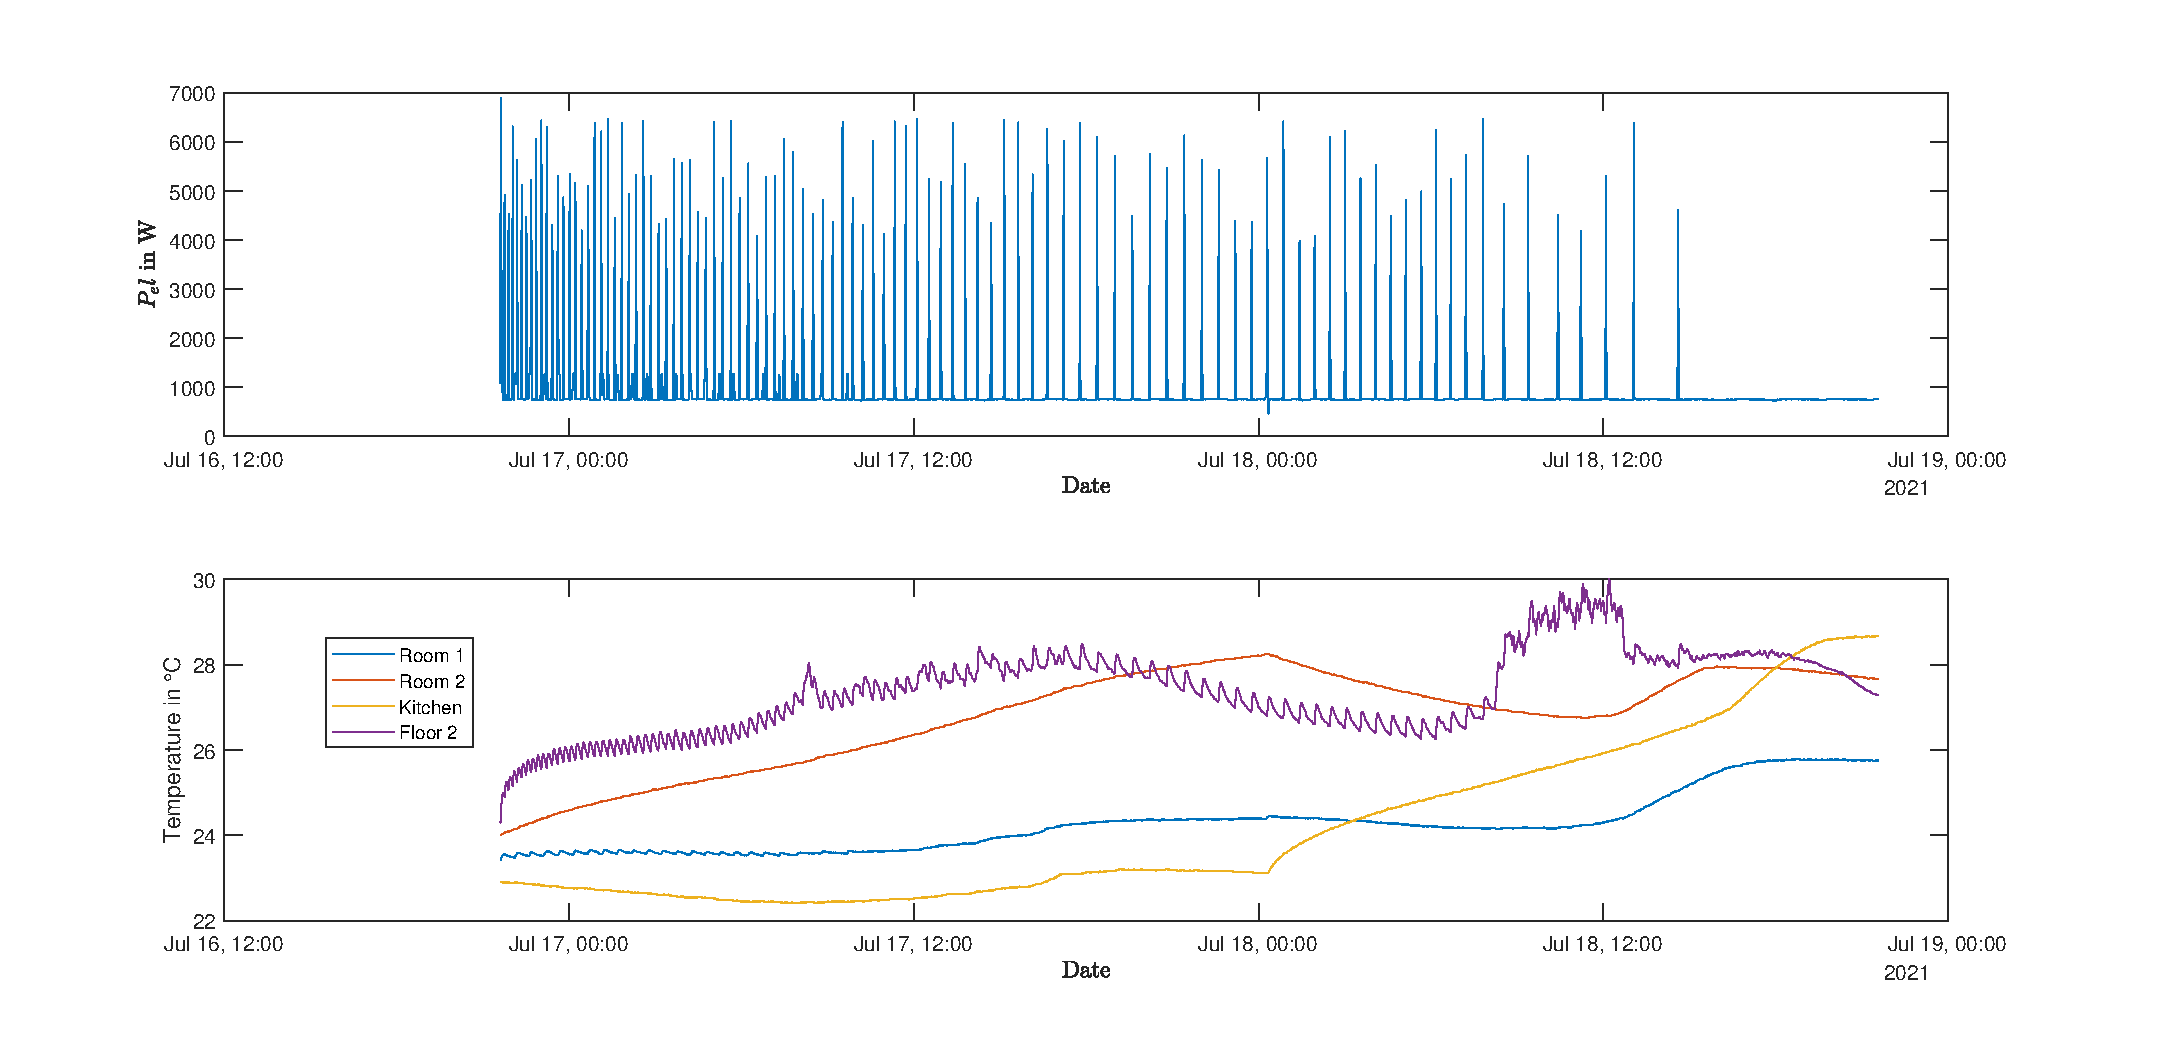
\includegraphics[width=0.85\textwidth]{figure/P_el_trainingsdaten_latex.eps}
           \caption{Electrical consumption of the building and air temperature inside the rooms during the experiment 1}
           \label{fig:P_elTemperatureExperiment1}
    \end{figure}
\section{Experiment 2}
\label{sec:Experiment2}
Experiment 2 roots also on the general assumption of converting the entire electrical power to heat, and starts on Monday, 26. July 2021 and ends on Sunday night, 1. August 2021. We use also the heaters explained in \autoref{tab:HeatersData}. In contrast to experiment 1, we can now remotely control the switching on and off of the heaters due to an update in the building. Therefore, we can generate more training data by controlling heating periods on working days during the night and on the weekend. In order not to burden the occupants during the working day, we heat at night and only the unused kitchen with the HoHeF. In addition, we can use another measuring point for the electrical consumption during the working days, where the electric car charging is not considered. Only for the weekend, we need both measuring points (the one only used in experiment 1 and the new one used during the working days in experiment 2) to measure the whole energy consumption because of the three-phase connection of the IH, which is measured at the same point as car charging. So, we have to ensure no car charging during the weekend. Besides, the heaters are in the same rooms as in experiment 1 over the weekend. \autoref{tab:Experiment2app} or the data describe the incidences during experiment 2, which is explained in detail in the next section. 

\subsection{Data of the experiment 2}
\label{subsec:Data of the experiment 2}
\autoref{fig:P_elTemperatureExperiment2} presents the needed electrical consumption and the air temperatures of the rooms of interest during experiment 2. Especially, the air temperature of the kitchen is showed over the whole experimental phase because in the first five days only this room is heated for reasons explained above. The heating periods are remarked by horizontal lines. The visible horizontal curves of the air temperatures arise from the breakdown of the programmable logic controller (PLC) \nomenclature[A]{PLC}{Programmable Logic Controller}. During this breakdown, no temperature data can be recorded. In every heating period with a working PLC, the increasing temperatures are conspicuous. Notice the third period: The rising temperature is visible from the point at closing the door in the kitchen (compare \autoref{tab:Experiment2app}). When the door is open, the heat spreads in the building and, a smaller temperature rise is visible in the kitchen.  In this experiment, also, the different heaters have the same effect on the air temperatures and the HoHeF is moved from room 2 to the kitchen to avoid too high temperatures at the weekend.
\begin{figure}[H]
            \centering
            %\def\svgwidth{100pt}
            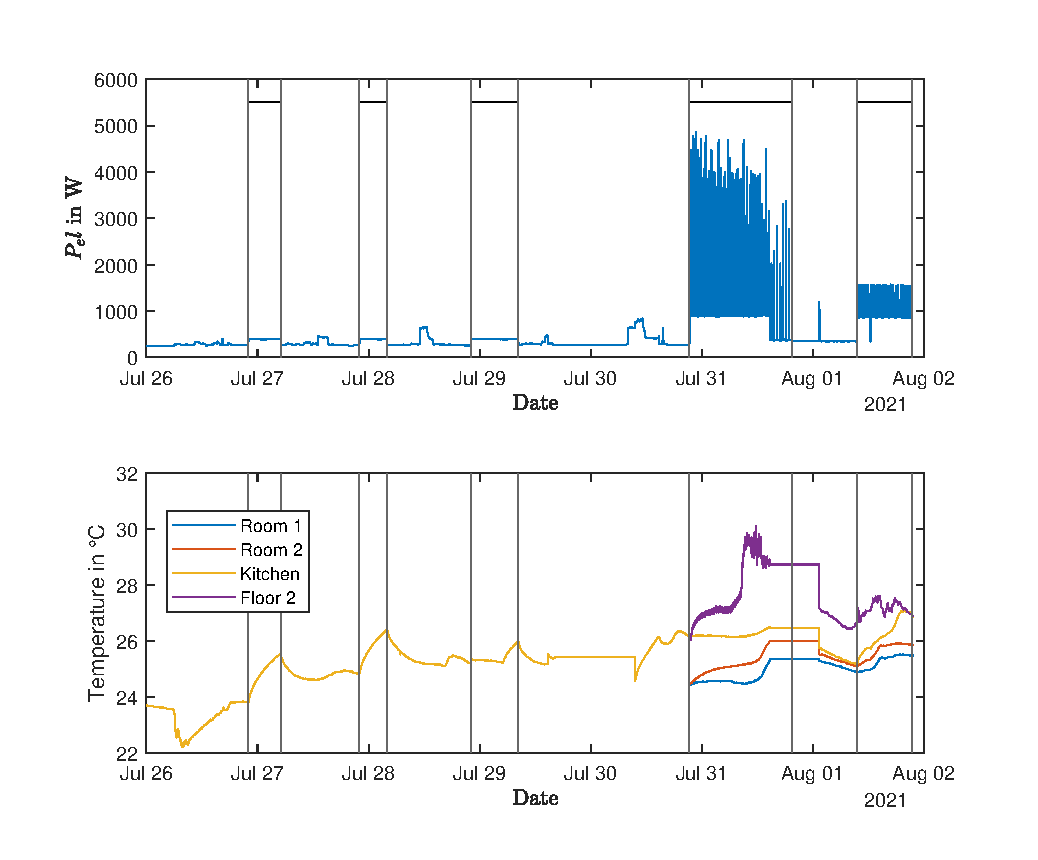
\includegraphics[width=0.85\textwidth]{figure/Trainingsdaten_P_el_und_Raumtemperaturen_latex.eps}
           \caption{Electrical consumption of the building and air temperature inside the rooms during the experiment 2}
           \label{fig:P_elTemperatureExperiment2}
\end{figure}

\section{Findings of the experiments}
\label{sec:findings of the experiments}
All influences on the building are noticeable in the data. The heating of a room directly increases the air temperature and with a time delay the wall and screed temperatures; the room temperature rises more slowly through open inner doors; the temperature curves show whether the heating is heating or not; and opening all windows and doors lead to a decreasing temperature at the end of the experiments. \newline
No temperature data can be recorded during the PLC breakdown. This degrades the quality of the data used to estimate the model. Especially during this time, it is partially heated. Data collection would be particularly important here to determine the influence of heating. To reduce the negative impact on the data, it is important to switch off the heaters quickly in case of PLC breakdown, which is possible with remote access for the household heaters. This does not apply to the IH, as it has no remote control due to its three-phase connection and thus heats for longer periods without temperature detection.\newline
In a look back, the use of different measuring points for electrical consumption is disadvantageous. If it seemed advantageous when considering experiment 2 that no consideration has to be given to the car charging, this actually means that the same combination of measuring points has to be used for the verification data from experiment 1, which was not planned, at first.\newline

